\documentclass[12pt,a4paper]{report}

% Packages
\usepackage[utf8]{inputenc}
\usepackage[T1]{fontenc}
\usepackage{times}
\usepackage[margin=1in]{geometry}
\usepackage{graphicx}
\usepackage{booktabs}
\usepackage{longtable}
\usepackage{array}
\usepackage{multirow}
\usepackage{float}
\usepackage{caption}
\usepackage{hyperref}
\usepackage{listings}
\usepackage{xcolor}
\usepackage{tikz}
\usetikzlibrary{shapes.geometric, arrows, positioning}
\usepackage{setspace}
\usepackage{titlesec}
\usepackage{fancyhdr}
\usepackage{enumitem}

% Page style
\pagestyle{fancy}
\fancyhf{}
\fancyhead[L]{\leftmark}
\fancyhead[R]{\thepage}
\renewcommand{\headrulewidth}{0.4pt}

% Line spacing
\onehalfspacing

% Hyperref setup
\hypersetup{
    colorlinks=true,
    linkcolor=blue,
    filecolor=magenta,
    urlcolor=cyan,
    citecolor=blue
}

\begin{document}

% Title Page
\begin{titlepage}
    \centering
    \vspace*{2cm}
    {\Huge\bfseries PIXELAR\\[0.5cm]}
    {\Large An AI-Powered Platform for Automated 2D Game Asset Generation\\[2cm]}
    {\large\bfseries Technical Documentation\\[0.5cm]}
    {\normalsize Prepared in Accordance with IEEE Standards\\[3cm]}
    \vfill
    {\large \today}
\end{titlepage}

% Abstract
\begin{abstract}
This document presents the technical documentation for Pixelar, an innovative web-based platform designed to facilitate the automated generation of two-dimensional game assets through artificial intelligence technologies. The platform addresses the significant challenges faced by game developers, particularly independent creators and small studios, in producing high-quality visual assets. By leveraging state-of-the-art diffusion models and providing an integrated workflow for sprite, scene, and animation generation, Pixelar aims to democratize access to professional-quality game art. This documentation encompasses the system overview, background research, requirements specification, architectural design, and testing methodology, all prepared in accordance with IEEE software engineering standards.
\end{abstract}

% Table of Contents
\tableofcontents
\newpage
\listoffigures
\newpage
\listoftables
\newpage


%==============================================================================
% CHAPTER 1: INTRODUCTION
%==============================================================================
\chapter{Introduction}

This chapter provides a comprehensive introduction to the Pixelar project, encompassing the system overview, project motivation, vision statement, scope definition, problem statement, objectives, development tools, and terminology definitions.

\section{System Overview}

Pixelar constitutes an innovative web-based application engineered to transform the creation of two-dimensional game assets through the application of artificial intelligence technologies. The platform provides game developers, independent studios, and pixel artists with sophisticated AI-driven tools capable of generating high-quality sprites, scenes, and animations suitable for integration with prevalent game engines, including Unity, Godot, and Unreal Engine.

The application leverages contemporary web technologies in conjunction with state-of-the-art AI image generation models to deliver a seamless creative experience. The system architecture comprises a Next.js-based frontend and an Express.js backend, enabling real-time asset generation, comprehensive project management capabilities, and extensive export options tailored for game development workflows.

The core functionality is organized into three primary asset generation modules:
\begin{itemize}
    \item \textbf{Sprite Generation Module}: Facilitates the creation of character sprites and game objects with configurable parameters including art style, viewpoint orientation, and color palette specifications.
    \item \textbf{Scene Generation Module}: Enables the production of background environments and game worlds for both indoor and outdoor settings.
    \item \textbf{Animation Generation Module}: Supports the creation of frame-by-frame character animations with pose control mechanisms and predefined animation type libraries.
\end{itemize}

Each module incorporates customizable parameters including art style selection (Pixel Art, 2D Flat), viewpoint configuration (Front, Back, Side, Top-Down, Isometric), color palette management, and aspect ratio control.

Pixelar addresses a significant gap in the game development toolchain by democratizing access to professional-quality game art. Traditional game asset creation necessitates extensive artistic expertise and considerable time investment. Through AI-powered generation, Pixelar enables developers to rapidly prototype and produce game-ready assets, thereby significantly reducing development cycles and lowering barriers to entry for independent game creators.

The platform implements a credit-based monetization system supporting multiple subscription tiers (Free, Pro, Enterprise), with an innovative Bring Your Own Key (BYOK) feature that permits users to utilize their personal API keys for AI generation services. This flexibility ensures accessibility for hobbyist developers while providing scalable solutions for professional studios.

\section{Project Motivation}

The video game industry has experienced unprecedented growth, with the global market valuation exceeding \$200 billion USD and demonstrating continued expansion \cite{newzoo2024}. Within this landscape, two-dimensional games maintain significant relevance, particularly within the independent game sector, mobile gaming platforms, and retro-style productions. However, a persistent challenge confronting game developers is the creation of visual assets, which traditionally requires either substantial artistic expertise or significant financial investment in professional artists.

Several key factors motivated the development of the Pixelar platform:

\textbf{The Democratization Paradox}: The democratization of game development tools has created a paradox wherein programming capabilities and game engine access have become increasingly accessible, yet visual asset creation remains a significant bottleneck. Game engines such as Unity and Godot provide free tiers, and numerous educational resources enable aspiring developers to acquire game programming skills. However, the creation of professional-quality sprites, backgrounds, and animations continues to require years of artistic training or expensive outsourcing arrangements.

\textbf{Emergence of Generative AI Technologies}: The emergence of generative AI technologies, particularly diffusion models and large language models, has opened new possibilities for automated content creation. Models such as Stable Diffusion and various proprietary APIs have demonstrated remarkable capabilities in generating images from textual descriptions \cite{rombach2022}. Pixelar harnesses these technologies specifically for game asset creation, optimizing prompts and workflows for pixel art and 2D game aesthetics.

\textbf{Underserved Independent Developer Market}: The independent game development community represents a substantial and underserved market segment. Independent developers frequently operate with limited budgets and small teams, rendering professional art assets financially prohibitive. Pixelar addresses this need by providing affordable, AI-generated alternatives that maintain quality standards suitable for commercial releases.

\textbf{Rapid Prototyping Requirements}: Time-to-market pressures in game development necessitate rapid prototyping capabilities. Even studios with dedicated art teams benefit from tools capable of quickly generating placeholder assets or exploring visual concepts prior to committing to full production. Pixelar serves both as a production tool and a rapid prototyping solution.

\textbf{Industry Acceptance of AI-Generated Content}: The growing acceptance of AI-generated content in creative industries signals a paradigm shift in digital asset production methodologies. Rather than replacing human artists, AI tools increasingly serve as force multipliers, enabling artists to work more efficiently and explore creative directions that would otherwise be impractical.


\section{Project Vision}

Pixelar envisions establishing itself as the premier platform for AI-assisted 2D game asset creation, thereby establishing a new paradigm in game development workflows. The project aims to achieve the following objectives:

\begin{enumerate}
    \item \textbf{Creator Empowerment}: Enable creators of all skill levels to produce professional-quality game assets without requiring traditional artistic training.
    \item \textbf{Industry Standard Establishment}: Establish industry-standard workflows for AI-generated game assets, including optimized export formats, sprite sheet generation, and animation frame management.
    \item \textbf{Community Development}: Foster a community of game developers who leverage AI tools responsibly and creatively.
    \item \textbf{Continuous Technological Evolution}: Continuously evolve with advancing AI technologies, incorporating new models and capabilities as they become available.
    \item \textbf{Ecosystem Support}: Support the broader game development ecosystem by providing tools that complement rather than compete with traditional asset creation methods.
\end{enumerate}

\section{Scope}

The scope of the Pixelar platform encompasses the following functional domains:

\subsection{In-Scope Features}

\textbf{1. AI-Powered Asset Generation}
\begin{itemize}
    \item Sprite generation for characters and objects with configurable parameters
    \item Scene and background generation for game environments
    \item Animation frame generation with pose control and frame descriptions
    \item Support for multiple art styles (Pixel Art, 2D Flat)
    \item Multiple viewpoint options (Front, Back, Side, Top-Down, Isometric)
\end{itemize}

\textbf{2. Project Management Functionality}
\begin{itemize}
    \item User project creation and organizational capabilities
    \item Asset storage and retrieval mechanisms
    \item Project categorization (Sprite projects, Scene projects)
    \item Thumbnail management and preview capabilities
\end{itemize}

\textbf{3. User Management System}
\begin{itemize}
    \item Firebase-based authentication (Google Sign-In)
    \item User profile management functionality
    \item Credit-based usage tracking system
    \item Multiple subscription tiers (Free, Pro, Enterprise)
\end{itemize}

\textbf{4. Export and Integration Capabilities}
\begin{itemize}
    \item PNG image export for individual assets
    \item Sprite sheet generation for animations
    \item GIF export for animated content
    \item Game engine-compatible format support
\end{itemize}

\textbf{5. Utility Tools}
\begin{itemize}
    \item Sprite sheet to GIF converter
    \item Animation frame editor
    \item 3D pose editor for character positioning
    \item Color palette management system
\end{itemize}

\subsection{Out-of-Scope Features}

The following features are explicitly excluded from the current project scope:
\begin{itemize}
    \item Three-dimensional asset generation and modeling
    \item Audio and sound effect generation
    \item Game logic or code generation
    \item Direct game engine plugins (assets are exported as standard formats)
    \item Collaborative real-time editing functionality
    \item Mobile application development (web-only platform)
\end{itemize}

\section{Problem Statement}

Game developers, particularly independent creators and small studios, encounter significant challenges in producing high-quality two-dimensional visual assets for their projects. The traditional approaches to obtaining game art present substantial barriers that impede development progress:

\textbf{Financial Barriers}: The engagement of professional pixel artists or 2D artists necessitates significant financial investment, frequently ranging from hundreds to thousands of dollars per asset. For independent developers operating with limited budgets, such costs prove prohibitive.

\textbf{Skill Requirements}: The acquisition of traditional digital art skills requires years of dedicated practice and training. While many developers possess strong programming abilities, the artistic skills necessary for professional game art represent a distinct discipline that cannot be rapidly acquired.

\textbf{Lack of Visual Uniqueness}: The utilization of pre-made asset packs, while cost-effective, results in games that lack visual uniqueness. Numerous independent games share identical or similar assets, thereby diminishing their market differentiation potential.

\textbf{Suboptimal AI Tool Availability}: Existing AI image generation tools, while powerful, are not optimized for game asset creation. General-purpose AI art generators produce images that require significant post-processing to achieve suitability for game integration.

\textbf{Workflow Fragmentation}: The absence of integrated workflows necessitates that developers navigate multiple tools and manual processes to convert AI-generated images into usable game assets.

These challenges collectively result in delayed development timelines, compromised visual quality, or abandoned projects when developers cannot overcome the art asset barrier.


\section{Objectives}

\subsection{Primary Objectives}

The primary objectives of the Pixelar project are as follows:

\begin{enumerate}
    \item To develop an intuitive web-based platform that enables users to generate game-ready 2D assets utilizing AI technology with minimal technical expertise requirements.
    \item To implement robust AI integration supporting multiple generation providers (Replicate API, Google Gemini) with optimized prompting mechanisms for game asset aesthetics.
    \item To create comprehensive project management functionality permitting users to organize, store, and retrieve generated assets efficiently.
    \item To design and implement a scalable credit-based monetization system supporting multiple user tiers while maintaining accessibility for hobbyist developers.
    \item To provide specialized tools for animation creation including frame generation, sprite sheet compilation, and GIF export capabilities.
\end{enumerate}

\subsection{Secondary Objectives}

The secondary objectives of the project include:

\begin{enumerate}
    \item To ensure cross-platform compatibility through responsive web design accessible from desktop and tablet devices.
    \item To implement secure authentication and data protection utilizing industry-standard practices.
    \item To optimize application performance for responsive user experience during asset generation and preview operations.
    \item To create extensible architecture permitting future integration of additional AI models and generation capabilities.
    \item To develop comprehensive export options compatible with major game engines (Unity, Godot, Unreal Engine).
\end{enumerate}

\subsection{Technical Objectives}

The technical objectives are specified as follows:

\begin{enumerate}
    \item To achieve sub-second response times for user interface interactions and asset previews.
    \item To maintain 99\% uptime for core generation services.
    \item To support concurrent users without degradation in service quality.
    \item To implement efficient blob storage for user assets with appropriate retention policies.
    \item To ensure secure handling of user API keys for BYOK functionality.
\end{enumerate}

\section{Development Tools and Technologies}

This section presents the tools and technologies utilized in the development and operation of the Pixelar platform.

\begin{table}[H]
\centering
\caption{Frontend Technologies}
\label{tab:frontend-tech}
\begin{tabular}{ll}
\toprule
\textbf{Technology} & \textbf{Purpose} \\
\midrule
Next.js 15 & React-based framework for server-side rendering \\
React 19 & JavaScript library for building user interfaces \\
TypeScript & Typed superset of JavaScript for type safety \\
Tailwind CSS & Utility-first CSS framework for styling \\
Radix UI & Unstyled, accessible component primitives \\
Three.js & 3D graphics library for pose editor implementation \\
GIF.js & Client-side GIF encoding library \\
Lucide React & Icon library for user interface elements \\
\bottomrule
\end{tabular}
\end{table}

\begin{table}[H]
\centering
\caption{Backend Technologies}
\label{tab:backend-tech}
\begin{tabular}{ll}
\toprule
\textbf{Technology} & \textbf{Purpose} \\
\midrule
Node.js & JavaScript runtime environment \\
Express.js & Web application framework for API development \\
TypeScript & Type-safe backend development \\
Firebase Admin SDK & Server-side Firebase integration \\
Zod & TypeScript-first schema validation library \\
\bottomrule
\end{tabular}
\end{table}

\begin{table}[H]
\centering
\caption{Database, Storage, and External Services}
\label{tab:services}
\begin{tabular}{ll}
\toprule
\textbf{Service} & \textbf{Purpose} \\
\midrule
Firebase Firestore & NoSQL document database for data persistence \\
Vercel Blob & Object storage for generated image assets \\
Firebase Authentication & User authentication with Google Sign-In \\
Replicate API & Primary AI image generation service \\
Google Gemini API & Alternative AI generation provider \\
\bottomrule
\end{tabular}
\end{table}

\begin{table}[H]
\centering
\caption{Development and Deployment Tools}
\label{tab:dev-tools}
\begin{tabular}{ll}
\toprule
\textbf{Tool} & \textbf{Purpose} \\
\midrule
Jest & JavaScript testing framework \\
ESLint & Code linting and style enforcement \\
Git & Version control system \\
Vercel & Frontend hosting and deployment platform \\
Firebase Cloud Run & Backend API hosting service \\
\bottomrule
\end{tabular}
\end{table}

\section{Glossary of Terms}

Table \ref{tab:glossary} presents definitions of technical terms and acronyms utilized throughout this documentation.

\begin{table}[H]
\centering
\caption{Glossary of Terms}
\label{tab:glossary}
\small
\begin{tabular}{p{3cm}p{10cm}}
\toprule
\textbf{Term} & \textbf{Definition} \\
\midrule
AI Generation & The process of creating images utilizing artificial intelligence models based on textual prompts \\
Animation Frame & A single image in a sequence that creates the illusion of movement when displayed in rapid succession \\
API Key & A unique identifier utilized to authenticate requests to external services \\
Aspect Ratio & The proportional relationship between an image's width and height dimensions \\
Asset & Any digital resource utilized in game development \\
BYOK & Bring Your Own Key; a feature permitting users to utilize personal API keys \\
Credit & Virtual currency unit utilized to track AI generation usage \\
Diffusion Model & An AI model that generates images by iteratively denoising random noise patterns \\
Firebase & Google's platform providing authentication and database services \\
Firestore & Firebase's NoSQL document database service \\
GIF & Graphics Interchange Format; an animated image format \\
Isometric View & Visual representation depicting 3D objects in 2D at a 45-degree angle \\
JWT & JSON Web Token; a secure method for transmitting authentication information \\
Pixel Art & Digital art style characterized by visible pixels as a deliberate aesthetic choice \\
Pose & The position and orientation of a character's body parts \\
Prompt & Textual description provided to AI models to guide image generation \\
Replicate & Cloud platform for executing machine learning models via API \\
Scene & A background or environment image for utilization in games \\
Sprite & A 2D image integrated into a game, typically representing characters or objects \\
Sprite Sheet & A single image containing multiple animation frames arranged in a grid \\
Token & Authentication credential utilized to verify user identity \\
Vercel Blob & Object storage service for hosting files \\
Viewpoint & The camera angle from which an asset is rendered \\
\bottomrule
\end{tabular}
\end{table}


%==============================================================================
% CHAPTER 2: BACKGROUND STUDY
%==============================================================================
\chapter{Background Study}

This chapter presents a comprehensive review of relevant prior research and existing solutions in the domains of AI-powered content generation, game asset creation tools, and web application development. Following detailed analysis, a comparative evaluation of discussed works is presented, along with identification of their limitations.

\section{Introduction}

The development of Pixelar is informed by extensive research into existing solutions, academic literature, and industry practices in the domains of AI-powered content generation, game asset creation tools, and web application development. This chapter presents a comprehensive analysis of relevant prior work, identifying both achievements and limitations that have shaped the design decisions for the Pixelar platform.

The background study encompasses three primary research areas:
\begin{enumerate}
    \item Existing AI image generation platforms and their applicability to game development
    \item Traditional and modern game asset creation tools
    \item Technical frameworks for building scalable web applications with AI integration
\end{enumerate}

\section{AI Image Generation Technologies}

The field of AI image generation has undergone rapid advancement since the introduction of Generative Adversarial Networks (GANs) by Goodfellow et al. in 2014 \cite{goodfellow2014}. Subsequent developments have produced increasingly sophisticated models capable of generating high-quality images from textual descriptions.

\subsection{Generative Adversarial Networks}

Generative Adversarial Networks introduced the concept of adversarial training, wherein a generator network creates images while a discriminator network evaluates their authenticity. This approach produced significant improvements in image generation quality. Notable GAN variants include:

\begin{itemize}
    \item \textbf{StyleGAN} \cite{karras2019}: Enabled fine-grained control over generated image attributes through style-based architecture, permitting manipulation of specific visual features.
    \item \textbf{BigGAN}: Demonstrated high-fidelity image generation at scale utilizing class-conditional generation mechanisms.
\end{itemize}

However, GANs presented several limitations for practical applications:
\begin{itemize}
    \item Training instability requiring careful hyperparameter tuning
    \item Mode collapse resulting in limited variety of outputs
    \item Difficulty in controlling specific image attributes through textual prompts
\end{itemize}

\subsection{Diffusion Models}

Diffusion models, particularly Denoising Diffusion Probabilistic Models (DDPMs) introduced by Ho et al. \cite{ho2020}, represent the current state-of-the-art in image generation. These models learn to reverse a gradual noising process, generating images by iteratively denoising random noise patterns.

The introduction of latent diffusion models by Rombach et al. \cite{rombach2022}, implemented in Stable Diffusion, dramatically improved computational efficiency by operating in a compressed latent space rather than pixel space.

Key advantages of diffusion models for the Pixelar use case include:
\begin{itemize}
    \item Superior text-to-image alignment compared to GAN-based approaches
    \item Stable training without mode collapse phenomena
    \item Ability to incorporate conditioning signals (text, images, poses)
    \item Active open-source development and model availability
\end{itemize}

\subsection{Commercial AI Generation Platforms}

Several commercial platforms have emerged offering AI image generation services:

\textbf{DALL-E (OpenAI)}: Pioneered text-to-image generation with impressive results; however, it operates as a closed system with limited customization options. Pricing models and usage restrictions limit applicability for high-volume game asset generation.

\textbf{Midjourney}: Gained popularity for artistic image generation with distinctive aesthetic qualities. However, the Discord-based interface and focus on artistic rather than technical outputs render it suboptimal for game asset workflows.

\textbf{Stable Diffusion (Stability AI)}: Open-source model enabling self-hosting and customization. The availability through APIs (including Replicate) renders it suitable for integration into custom applications such as Pixelar.

\textbf{Google Gemini}: Multimodal AI model with image generation capabilities, offering an alternative API for generation services with different strengths in prompt interpretation.

\section{Existing Game Asset Creation Tools}

\subsection{Traditional Digital Art Software}

Professional game artists typically utilize established digital art applications:

\textbf{Adobe Photoshop}: Industry-standard raster graphics editor with extensive features; however, it presents a steep learning curve and subscription costs. While powerful, it requires significant artistic skill to produce quality game assets.

\textbf{Aseprite}: Specialized pixel art editor popular among independent developers, offering animation timeline and sprite sheet export functionality. While excellent for manual creation, it provides no AI assistance capabilities.

\textbf{Pyxel Edit}: Tile-based pixel art editor focused on game development workflows, supporting tilemap creation and animation functionality.

\textbf{GraphicsGale}: Free pixel art animation software with frame management capabilities.

These tools require significant artistic skill and time investment, representing the traditional approach that Pixelar aims to complement.

\subsection{AI-Assisted Art Tools}

Recent developments have introduced AI capabilities to creative software:

\textbf{Adobe Firefly}: Integrated into Adobe products, offering generative fill and image generation. However, outputs are not optimized for game assets and require significant post-processing.

\textbf{Canva AI}: Provides AI image generation within a design platform; however, it lacks game-specific features and export options.

\textbf{Scenario.gg}: A platform specifically targeting game asset generation with AI, offering training of custom models on existing art styles. This represents the closest existing solution to Pixelar's objectives, albeit with different technical approaches and pricing models.

\textbf{Leonardo.AI}: Provides AI image generation with some game-focused features, including model fine-tuning capabilities.


\section{Animation Generation Research}

Character animation generation represents a specialized challenge within AI content creation.

\subsection{Pose-Guided Generation}

ControlNet, introduced by Zhang et al. \cite{zhang2023}, introduced conditioning mechanisms for diffusion models, enabling pose-guided image generation. By providing skeletal pose information, users can control character positioning in generated images. This technology underlies Pixelar's animation frame generation approach.

\subsection{Video and Animation Synthesis}

Research into video generation models (Make-A-Video, Imagen Video) demonstrates potential for direct animation synthesis. However, current models lack the frame-level control and consistency required for game sprite animations, rendering frame-by-frame generation with pose guidance more practical for Pixelar's use case.

\subsection{Sprite Animation Datasets}

Academic datasets for sprite animation remain limited. The Sprites dataset and various game asset collections provide training data for specialized models, though most general-purpose image generation models lack specific training on pixel art animations.

\section{Web Application Architecture Research}

\subsection{Modern Frontend Frameworks}

The evolution of frontend frameworks has produced several options for building interactive web applications:

\textbf{React}: Component-based library enabling declarative UI development. Extensive ecosystem and community support render it suitable for complex applications.

\textbf{Next.js}: React framework adding server-side rendering, routing, and optimization features. Particularly suitable for applications requiring both static and dynamic content.

\textbf{Vue.js and Svelte}: Alternative frameworks with different paradigms, each presenting trade-offs in learning curve, performance, and ecosystem maturity.

\subsection{Backend API Design}

RESTful API design principles, as established by Fielding \cite{fielding2000}, provide the foundation for Pixelar's backend architecture. Additional considerations include:
\begin{itemize}
    \item Authentication patterns utilizing JWT tokens and OAuth 2.0 flows
    \item Rate limiting and quota management for AI service integration
    \item Asynchronous processing for long-running generation tasks
    \item Caching strategies for frequently accessed resources
\end{itemize}

\subsection{Cloud Storage Solutions}

Research into object storage services (AWS S3, Google Cloud Storage, Vercel Blob) informed the selection of Vercel Blob for asset storage, considering factors including:
\begin{itemize}
    \item Integration simplicity with the deployment platform
    \item Cost structure for storage and bandwidth
    \item CDN capabilities for global asset delivery
    \item API design for programmatic access
\end{itemize}


\section{Comparative Analysis of Related Works}

Table \ref{tab:comparison} presents a comparative analysis of existing solutions related to Pixelar's functionality.

\begin{table}[H]
\centering
\caption{Comparative Analysis of Game Asset Generation Tools}
\label{tab:comparison}
\small
\begin{tabular}{lccccc}
\toprule
\textbf{Feature} & \textbf{Pixelar} & \textbf{Scenario} & \textbf{Leonardo} & \textbf{Midjourney} & \textbf{Aseprite} \\
\midrule
AI Image Generation & Yes & Yes & Yes & Yes & No \\
Game Optimization & Yes & Yes & Partial & No & N/A \\
Pixel Art Style & Yes & Yes & Yes & Limited & Manual \\
Animation Generation & Yes & Limited & No & No & Manual \\
Sprite Sheet Export & Yes & Yes & No & No & Yes \\
Project Management & Yes & Yes & Yes & No & Local \\
BYOK Support & Yes & No & No & No & N/A \\
Web-Based Interface & Yes & Yes & Yes & Discord & Desktop \\
Free Tier Availability & Yes & Limited & Yes & No & One-time \\
Custom Pose Control & Yes & No & Limited & No & Manual \\
Real-time Preview & Yes & Yes & Yes & No & Yes \\
\bottomrule
\end{tabular}
\end{table}

The comparative analysis reveals that while several platforms address portions of the game asset creation challenge, no single existing solution provides the comprehensive feature set that Pixelar offers, particularly in the areas of animation generation with pose control and BYOK support.

\section{Limitations of Existing Solutions}

Analysis of existing solutions reveals several limitations that Pixelar addresses:

\subsection{General AI Image Generators}

Platforms such as DALL-E, Midjourney, and Stable Diffusion Web present the following limitations:

\begin{enumerate}
    \item \textbf{Lack of Game-Specific Optimization}: Generated images require manual post-processing for game integration, including background removal, resizing, and format conversion.
    \item \textbf{Absence of Animation Workflow}: These platforms generate single images without support for creating animation sequences or maintaining character consistency across frames.
    \item \textbf{Limited Export Options}: Standard image downloads without sprite sheet generation, transparency handling, or game engine-specific formats.
    \item \textbf{No Project Organization}: Generated images are not organized into projects or associated with metadata useful for game development.
\end{enumerate}

\subsection{Specialized Game Asset Tools}

Platforms such as Scenario.gg present the following limitations:

\begin{enumerate}
    \item \textbf{Pricing Barriers}: Professional features frequently require expensive subscriptions, limiting accessibility for independent developers.
    \item \textbf{Limited Animation Support}: While offering some animation features, comprehensive frame-by-frame generation with pose control remains limited.
    \item \textbf{No BYOK Option}: Users cannot leverage their own API keys to reduce costs or access specific models.
    \item \textbf{Platform Lock-in}: Assets and projects are tied to the platform without portable export options.
\end{enumerate}

\subsection{Traditional Art Software}

Tools such as Aseprite and Photoshop present the following limitations:

\begin{enumerate}
    \item \textbf{Skill Requirement}: Effective utilization requires significant artistic training and practice.
    \item \textbf{Time Investment}: Manual asset creation is time-consuming, particularly for animations requiring multiple frames.
    \item \textbf{No AI Assistance}: These tools provide no automated generation capabilities, relying entirely on user skill.
    \item \textbf{Cost Considerations}: Professional software requires ongoing subscription fees or significant one-time purchases.
\end{enumerate}


\section{Research Gaps Addressed by Pixelar}

Based on the background study, Pixelar addresses the following identified research and practical gaps:

\begin{enumerate}
    \item \textbf{Integrated Animation Workflow}: Unlike existing solutions, Pixelar provides end-to-end animation generation from pose selection through frame generation to sprite sheet export.
    \item \textbf{Accessible Pricing Model}: The credit-based system with BYOK support enables cost-effective usage for developers at all budget levels.
    \item \textbf{Game-Optimized Generation}: Prompt engineering and parameter optimization specifically target game asset aesthetics rather than general artistic output.
    \item \textbf{Comprehensive Project Management}: Integration of generation, storage, and organization within a unified platform streamlines the asset creation workflow.
    \item \textbf{Multiple AI Provider Support}: Flexibility to utilize different AI services (Replicate, Gemini) provides redundancy and permits users to select optimal providers for their requirements.
\end{enumerate}

\section{Theoretical Framework}

The design of Pixelar is grounded in several established theoretical frameworks:

\subsection{User-Centered Design}

Following Norman's principles of user-centered design \cite{norman2013}, the interface design prioritizes user needs and workflows, minimizing cognitive load while providing access to advanced features. Progressive disclosure presents basic options prominently while rendering advanced parameters accessible without overwhelming novice users.

\subsection{Agile Development Methodology}

The project follows agile principles with iterative development cycles, enabling rapid response to user feedback and evolving requirements. Feature prioritization based on user value guides development decisions.

\subsection{Microservices Architecture Principles}

While not a full microservices implementation, the separation of frontend, backend API, and external AI services follows principles of service isolation, enabling independent scaling and maintenance of system components.

\subsection{RESTful API Design}

Backend API design adheres to REST principles as established by Fielding \cite{fielding2000}, providing predictable, stateless endpoints that facilitate frontend development and potential future integrations.


\section{Summary}

The background study reveals a maturing landscape of AI image generation technologies with significant potential for game development applications. While existing solutions address portions of the game asset creation challenge, no single platform provides the comprehensive, accessible, and game-optimized solution that Pixelar aims to deliver.

Key findings informing Pixelar's development include:
\begin{itemize}
    \item Diffusion models (particularly Stable Diffusion) provide the most suitable foundation for game asset generation
    \item Animation generation requires specialized workflows beyond single-image generation
    \item Project management and export capabilities are essential for practical game development integration
    \item Pricing accessibility significantly impacts adoption among independent developers
    \item BYOK functionality addresses both cost concerns and user preference for specific AI providers
\end{itemize}

These findings directly inform the system requirements, architecture, and design decisions presented in Chapter 3.


%==============================================================================
% CHAPTER 3: SYSTEM REQUIREMENTS, ARCHITECTURE, AND DESIGN
%==============================================================================
\chapter{System Requirements, Architecture, and Design}

This chapter presents the functional requirements, non-functional requirements, system architecture, and design specifications for the Pixelar platform. The documentation adheres to IEEE Standard 830-1998 for Software Requirements Specifications \cite{ieee830}.

\section{System Flow Chart}

Figure \ref{fig:flowchart} illustrates the primary user workflow for asset generation in the Pixelar platform.

\begin{figure}[H]
	\centering
	\begin{tikzpicture}[node distance=0.7cm, auto,
		% UML Standard Shapes
		initial/.style={circle, fill=black, minimum size=0.4cm},
		final/.style={circle, draw=black, thick, minimum size=0.4cm, path picture={\fill[black] (path picture bounding box.center) circle (0.12cm);}},
		action/.style={rectangle, rounded corners=3pt, minimum width=2cm, minimum height=0.45cm, text centered, draw=black, fill=white, font=\scriptsize},
		decision/.style={diamond, minimum width=0.6cm, minimum height=0.6cm, draw=black, fill=white, inner sep=0pt},
		fork/.style={rectangle, fill=black, minimum width=1.2cm, minimum height=0.08cm},
		join/.style={rectangle, fill=black, minimum width=1.2cm, minimum height=0.08cm},
		arrow/.style={->,>=stealth, thick},
		guard/.style={font=\tiny}]
		
		% Initial Node
		\node (start) [initial] {};
		
		% Authentication
		\node (login) [action, below=of start] {Authenticate User};
		\node (d1) [decision, below=of login] {};
		\node (home) [action, below=of d1] {Display Dashboard};
		
		% Selection
		\node (select) [action, below=of home] {Select Generation Type};
		
		% Fork for generation types
		\node (fork1) [fork, below=of select] {};
		
		% Three parallel actions
		\node (sprite) [action, below left=0.6cm and 1cm of fork1] {Generate Sprite};
		\node (scene) [action, below=0.6cm of fork1] {Generate Scene};
		\node (anim) [action, below right=0.6cm and 1cm of fork1] {Generate Animation};
		
		% Join
		\node (join1) [join, below=1.8cm of fork1] {};
		
		% Configuration
		\node (config) [action, below=of join1] {Configure Parameters};
		
		% Credit Decision
		\node (d2) [decision, below=of config] {};
		\node (error) [action, right=1.5cm of d2] {Display Error};
		
		% AI Processing
		\node (api) [action, below=of d2] {Invoke AI Service};
		\node (store) [action, below=of api] {Store Generated Assets};
		\node (preview) [action, below=of store] {Display Preview};
		
		% Output Decision
		\node (d3) [decision, below=of preview] {};
		
		% Output Fork
		\node (fork2) [fork, below=of d3] {};
		\node (download) [action, below left=0.5cm and 0.8cm of fork2] {Download Asset};
		\node (save) [action, below=0.5cm of fork2] {Save to Project};
		\node (join2) [join, below=1.5cm of fork2] {};
		
		% Regenerate loop
		\node (regen) [action, right=1.5cm of d3] {Regenerate};
		
		% Final Node
		\node (end) [final, below=of join2] {};
		
		% Arrows
		\draw [arrow] (start) -- (login);
		\draw [arrow] (login) -- (d1);
		\draw [arrow] (d1) -- node[right, guard] {[valid]} (home);
		\draw [arrow] (d1.west) -- ++(-0.6,0) node[above, guard] {[invalid]} |- (login);
		\draw [arrow] (home) -- (select);
		\draw [arrow] (select) -- (fork1);
		
		% Fork arrows
		\draw [arrow] (fork1.south) -- ++(-1.5,0) |- (sprite.west);
		\draw [arrow] (fork1.south) -- (scene);
		\draw [arrow] (fork1.south) -- ++(1.5,0) |- (anim.east);
		
		% Join arrows
		\draw [arrow] (sprite.south) |- (join1.west);
		\draw [arrow] (scene) -- (join1);
		\draw [arrow] (anim.south) |- (join1.east);
		
		\draw [arrow] (join1) -- (config);
		\draw [arrow] (config) -- (d2);
		\draw [arrow] (d2) -- node[right, guard] {[sufficient]} (api);
		\draw [arrow] (d2) -- node[above, guard] {[insufficient]} (error);
		\draw [arrow] (error.north) |- (home);
		\draw [arrow] (api) -- (store);
		\draw [arrow] (store) -- (preview);
		\draw [arrow] (preview) -- (d3);
		
		% Output decision
		\draw [arrow] (d3) -- node[right, guard] {[export]} (fork2);
		\draw [arrow] (d3) -- node[above, guard] {[retry]} (regen);
		\draw [arrow] (regen.north) |- (config);
		
		% Final fork
		\draw [arrow] (fork2.south) -- ++(-0.8,0) |- (download.west);
		\draw [arrow] (fork2.south) -- (save);
		\draw [arrow] (download.south) |- (join2.west);
		\draw [arrow] (save) -- (join2);
		
		\draw [arrow] (join2) -- (end);
		
	\end{tikzpicture}
	\caption{UML Activity Diagram: Pixelar System Workflow}
	\label{fig:uml-activity}
\end{figure}

The flow chart demonstrates the sequential process from user authentication through asset generation and output handling. Key decision points include credit verification prior to generation and multiple output options following successful generation.


\section{Use Case Diagram}

Figure \ref{fig:usecase} illustrates the primary actors and their interactions with the Pixelar system.

\begin{figure}[H]
\centering
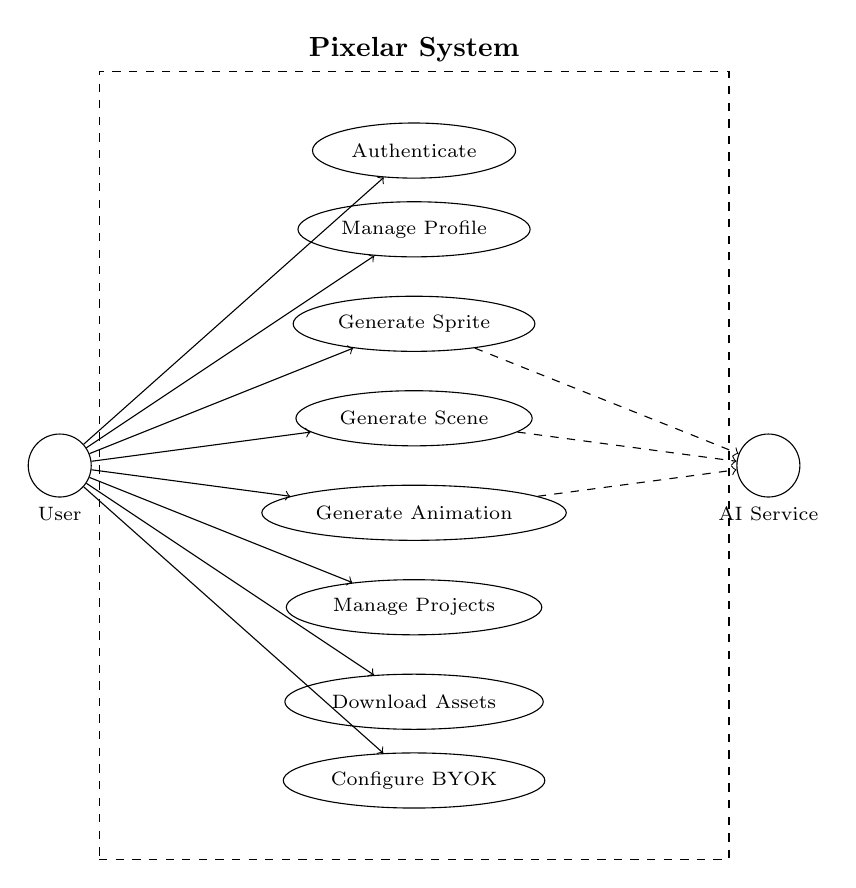
\begin{tikzpicture}[
    actor/.style={circle, draw, minimum size=0.8cm, font=\small},
    usecase/.style={ellipse, draw, minimum width=2cm, minimum height=0.7cm, text centered, font=\scriptsize},
    system/.style={rectangle, draw, dashed, minimum width=8cm, minimum height=10cm}
]

% System boundary
\node[system, label=above:{\textbf{Pixelar System}}] (system) at (4,0) {};

% Actor
\node[actor, label=below:{\scriptsize User}] (user) at (-0.5,0) {};

% Use cases
\node[usecase] (auth) at (4,4) {Authenticate};
\node[usecase] (profile) at (4,3) {Manage Profile};
\node[usecase] (sprite) at (4,1.8) {Generate Sprite};
\node[usecase] (scene) at (4,0.6) {Generate Scene};
\node[usecase] (anim) at (4,-0.6) {Generate Animation};
\node[usecase] (project) at (4,-1.8) {Manage Projects};
\node[usecase] (download) at (4,-3) {Download Assets};
\node[usecase] (byok) at (4,-4) {Configure BYOK};

% External actor
\node[actor, label=below:{\scriptsize AI Service}] (ai) at (8.5,0) {};

% Connections from user
\draw[->] (user) -- (auth);
\draw[->] (user) -- (profile);
\draw[->] (user) -- (sprite);
\draw[->] (user) -- (scene);
\draw[->] (user) -- (anim);
\draw[->] (user) -- (project);
\draw[->] (user) -- (download);
\draw[->] (user) -- (byok);

% Connections to AI service
\draw[dashed,->] (sprite) -- (ai);
\draw[dashed,->] (scene) -- (ai);
\draw[dashed,->] (anim) -- (ai);

\end{tikzpicture}
\caption{Use Case Diagram}
\label{fig:usecase}
\end{figure}

The use case diagram illustrates the primary actors (User, External AI Provider) and their interactions with the Pixelar system. The User actor represents authenticated users who can access all platform features. The External AI Provider represents the Replicate or Gemini API services utilized for image generation.

\section{Software Development Plan}

\subsection{System Architecture}

Pixelar employs a three-tier architecture separating presentation, business logic, and data management concerns. Figure \ref{fig:architecture} illustrates the system architecture.

\begin{figure}[H]
\centering
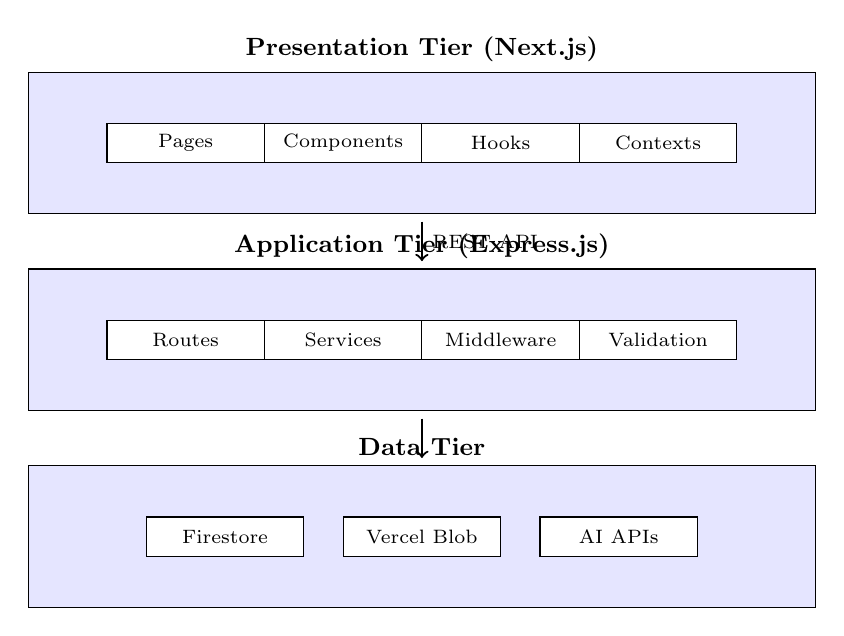
\begin{tikzpicture}[
    tier/.style={rectangle, draw, minimum width=10cm, minimum height=1.8cm, fill=blue!10},
    component/.style={rectangle, draw, minimum width=2cm, minimum height=0.5cm, fill=white, font=\scriptsize}
]

% Presentation Tier
\node[tier, label=above:{\small\textbf{Presentation Tier (Next.js)}}] (pres) at (0,4) {};
\node[component] at (-3,4) {Pages};
\node[component] at (-1,4) {Components};
\node[component] at (1,4) {Hooks};
\node[component] at (3,4) {Contexts};

% Application Tier
\node[tier, label=above:{\small\textbf{Application Tier (Express.js)}}] (app) at (0,1.5) {};
\node[component] at (-3,1.5) {Routes};
\node[component] at (-1,1.5) {Services};
\node[component] at (1,1.5) {Middleware};
\node[component] at (3,1.5) {Validation};

% Data Tier
\node[tier, label=above:{\small\textbf{Data Tier}}] (data) at (0,-1) {};
\node[component] at (-2.5,-1) {Firestore};
\node[component] at (0,-1) {Vercel Blob};
\node[component] at (2.5,-1) {AI APIs};

% Arrows
\draw[->, thick] (0,3) -- (0,2.5) node[midway, right, font=\scriptsize] {REST API};
\draw[->, thick] (0,0.5) -- (0,0);

\end{tikzpicture}
\caption{Three-Tier System Architecture}
\label{fig:architecture}
\end{figure}

\textbf{Presentation Tier}: The Next.js frontend handles all user interface rendering, client-side state management, and user interactions.

\textbf{Application Tier}: The Express.js backend provides RESTful API endpoints, implements business logic, handles authentication verification, and orchestrates interactions with external services.

\textbf{Data Tier}: Comprises Firebase Firestore for structured data storage, Vercel Blob for binary asset storage, and external AI APIs for generation services.

\subsection{Development Iterations}

The project follows an iterative development approach with the following planned iterations:

\begin{table}[H]
\centering
\caption{Development Iteration Schedule}
\label{tab:iterations}
\begin{tabular}{clp{7cm}}
\toprule
\textbf{Iteration} & \textbf{Duration} & \textbf{Focus Areas} \\
\midrule
1 & Weeks 1--3 & Project setup, authentication, basic UI, database schema \\
2 & Weeks 4--6 & Sprite generation, AI API integration, preview, credits \\
3 & Weeks 7--9 & Scene generation, animation, project management \\
4 & Weeks 10--11 & Sprite sheet converter, GIF export, animation tools \\
5 & Week 12 & Performance optimization, UI refinement, documentation \\
\bottomrule
\end{tabular}
\end{table}

\section{Fully Dressed Use Cases}

This section presents detailed use case specifications following the fully dressed format as recommended by Cockburn \cite{cockburn2001}.

\subsection{Use Case 1: Generate Sprite}

\textbf{Use Case ID:} UC-001

\textbf{Use Case Name:} Generate Sprite

\textbf{Primary Actor:} Authenticated User

\textbf{Stakeholders and Interests:}
\begin{itemize}
    \item \textit{User}: Requires high-quality sprite assets that meet specified parameters and are suitable for game development integration.
    \item \textit{System}: Manages computational resources efficiently, ensures proper credit deduction, and maintains data integrity.
\end{itemize}

\textbf{Preconditions:}
\begin{itemize}
    \item The user has successfully authenticated via Google Sign-In.
    \item The user possesses sufficient credits in their account (minimum 5 credits required).
    \item The system has active connectivity to the AI generation service (Replicate or Gemini API).
\end{itemize}

\textbf{Postconditions (Success Guarantee):}
\begin{itemize}
    \item Generated sprite images are displayed in the preview area.
    \item Credits have been deducted from the user's account.
    \item Asset records have been created in the database.
    \item Images have been uploaded to blob storage.
\end{itemize}

\textbf{Main Success Scenario:}
\begin{enumerate}
    \item User navigates to the Sprite Generator page.
    \item User selects sprite type (Character or Object).
    \item User enters a textual prompt describing the desired sprite.
    \item User configures generation parameters including art style, viewpoint, aspect ratio, and color palette.
    \item User optionally uploads a reference image for style guidance.
    \item User activates the ``Generate'' button.
    \item System validates that the user possesses sufficient credits.
    \item System constructs an optimized prompt and invokes the AI API.
    \item System receives generated images from the AI service.
    \item System uploads images to blob storage.
    \item System creates asset records in the database.
    \item System deducts credits from the user account.
    \item System displays generated sprites in the preview area.
    \item User may download assets, save to project, or initiate regeneration.
\end{enumerate}

\textbf{Extensions (Alternative Flows):}
\begin{itemize}
    \item \textit{7a. Insufficient credits:} System displays an error message indicating the required credits versus available credits. The use case terminates without credit deduction.
    \item \textit{8a. AI API error:} System displays an appropriate error message and does not deduct credits. User may retry the generation.
    \item \textit{9a. Generation timeout:} System implements automatic retry logic. If retry fails, system displays a timeout error message.
\end{itemize}

\textbf{Special Requirements:}
\begin{itemize}
    \item Generation request shall complete within 60 seconds.
    \item Generated images shall be stored with appropriate metadata for retrieval.
\end{itemize}

\textbf{Frequency of Occurrence:} High (primary system function)

\subsection{Use Case 2: Generate Animation}

\textbf{Use Case ID:} UC-002

\textbf{Use Case Name:} Generate Animation

\textbf{Primary Actor:} Authenticated User

\textbf{Stakeholders and Interests:}
\begin{itemize}
    \item \textit{User}: Requires consistent animation frames that can be compiled into sprite sheets for game integration.
    \item \textit{System}: Manages sequential frame generation efficiently and ensures character consistency across frames.
\end{itemize}

\textbf{Preconditions:}
\begin{itemize}
    \item The user has successfully authenticated via Google Sign-In.
    \item The user possesses sufficient credits (3 credits per frame $\times$ number of frames).
    \item A character reference image is available for animation generation.
\end{itemize}

\textbf{Postconditions (Success Guarantee):}
\begin{itemize}
    \item Animation frames have been generated and are displayed in the preview area.
    \item Animated preview is available for playback.
    \item Sprite sheet export functionality is enabled.
    \item Credits have been deducted from the user's account.
\end{itemize}

\textbf{Main Success Scenario:}
\begin{enumerate}
    \item User navigates to the Animation Generator page.
    \item User uploads a character reference image.
    \item User selects an animation type from the predefined library (e.g., Walking, Running, Attack).
    \item User selects view type (Isometric) and direction parameters.
    \item System displays frame descriptions for the selected animation type.
    \item User activates the ``Generate Animation'' button.
    \item System validates credit availability (3 credits per frame $\times$ number of frames).
    \item System generates each frame sequentially with appropriate pose descriptions.
    \item System compiles frames and displays an animated preview.
    \item System deducts credits from the user account.
    \item User may play or pause the animation preview.
    \item User may download as sprite sheet or individual frames.
\end{enumerate}

\textbf{Extensions (Alternative Flows):}
\begin{itemize}
    \item \textit{7a. Insufficient credits:} System calculates and displays the total credits required. The use case terminates without credit deduction.
    \item \textit{8a. Frame generation failure:} System logs the error and attempts regeneration of the failed frame. If persistent, partial results are displayed with error notification.
\end{itemize}

\textbf{Special Requirements:}
\begin{itemize}
    \item Character consistency shall be maintained across all generated frames.
    \item Sprite sheet export shall support configurable grid layouts.
\end{itemize}

\textbf{Frequency of Occurrence:} Medium

\subsection{Use Case 3: Manage Project}

\textbf{Use Case ID:} UC-003

\textbf{Use Case Name:} Manage Project

\textbf{Primary Actor:} Authenticated User

\textbf{Stakeholders and Interests:}
\begin{itemize}
    \item \textit{User}: Requires organizational capabilities to manage generated assets across multiple game development projects.
    \item \textit{System}: Maintains data integrity and enforces user-level data isolation.
\end{itemize}

\textbf{Preconditions:}
\begin{itemize}
    \item The user has successfully authenticated via Google Sign-In.
\end{itemize}

\textbf{Postconditions (Success Guarantee):}
\begin{itemize}
    \item Project is created, modified, or deleted as requested by the user.
    \item Project list is updated to reflect changes.
    \item Associated assets are properly linked or unlinked as appropriate.
\end{itemize}

\textbf{Main Success Scenario:}
\begin{enumerate}
    \item User navigates to the Projects page.
    \item User activates the ``New Project'' button.
    \item User enters a project name.
    \item User selects project type (Sprite or Scene).
    \item User activates the ``Create'' button.
    \item System creates a project record in the database.
    \item System displays the new project in the project list.
    \item User may open the project to view or add assets.
\end{enumerate}

\textbf{Extensions (Alternative Flows):}
\begin{itemize}
    \item \textit{3a. Duplicate project name:} System permits duplicate names but assigns unique identifiers internally.
    \item \textit{*a. Delete project:} User selects existing project and confirms deletion. System removes project record and disassociates linked assets.
\end{itemize}

\textbf{Special Requirements:}
\begin{itemize}
    \item Project deletion shall not delete associated assets from storage.
    \item Project thumbnails shall be automatically generated from the first associated asset.
\end{itemize}

\textbf{Frequency of Occurrence:} Medium

\section{System Sequence Diagram}

Figure \ref{fig:ssd} illustrates the system sequence diagram for the sprite generation process, depicting the message flow between User, Frontend, Backend, and AI API components.

\begin{figure}[H]
\centering
\begin{tikzpicture}[
    actor/.style={rectangle, draw, minimum width=1.2cm, minimum height=0.6cm, font=\scriptsize},
    arrow/.style={->, >=stealth, font=\tiny}
]

% Actors
\node[actor] (user) at (0,0) {User};
\node[actor] (frontend) at (3,0) {Frontend};
\node[actor] (backend) at (6,0) {Backend};
\node[actor] (ai) at (9,0) {AI API};

% Lifelines
\draw[dashed] (0,-0.4) -- (0,-10);
\draw[dashed] (3,-0.4) -- (3,-10);
\draw[dashed] (6,-0.4) -- (6,-10);
\draw[dashed] (9,-0.4) -- (9,-10);

% Messages
\draw[arrow] (0,-0.8) -- node[above] {1. Navigate} (3,-0.8);
\draw[arrow, dashed] (3,-1.2) -- node[above] {2. Display} (0,-1.2);

\draw[arrow] (0,-1.8) -- node[above] {3. Configure} (3,-1.8);

\draw[arrow] (3,-2.5) -- node[above] {4. POST /generate} (6,-2.5);

\draw[arrow] (6,-3.2) -- node[above] {5. Verify Token} (6.3,-3.2);
\draw[arrow, dashed] (6.3,-3.5) -- (6,-3.5);

\draw[arrow] (6,-4.2) -- node[above] {6. Check Credits} (6.3,-4.2);
\draw[arrow, dashed] (6.3,-4.5) -- (6,-4.5);

\draw[arrow] (6,-5.2) -- node[above] {7. Generate} (9,-5.2);
\draw[arrow, dashed] (9,-5.8) -- node[above] {8. Images} (6,-5.8);

\draw[arrow] (6,-6.5) -- node[above] {9. Store} (6.3,-6.5);
\draw[arrow, dashed] (6.3,-6.8) -- (6,-6.8);

\draw[arrow] (6,-7.5) -- node[above] {10. Deduct} (6.3,-7.5);
\draw[arrow, dashed] (6.3,-7.8) -- (6,-7.8);

\draw[arrow, dashed] (6,-8.5) -- node[above] {11. Response} (3,-8.5);

\draw[arrow, dashed] (3,-9.2) -- node[above] {12. Display} (0,-9.2);

\end{tikzpicture}
\caption{System Sequence Diagram for Sprite Generation}
\label{fig:ssd}
\end{figure}

The system sequence diagram illustrates the complete message flow for sprite generation, from user interaction through frontend processing, backend orchestration, external API invocation, and response handling. Key interactions include authentication verification, credit validation, AI API communication, and asset storage operations.

\section{Software Requirements Specification}

This section presents the functional and non-functional requirements for the Pixelar platform in accordance with IEEE Standard 830-1998 \cite{ieee830}.

\subsection{Functional Requirements}

\subsubsection{FR-001: User Authentication}

\textbf{FR-001.1:} The system shall support Google Sign-In authentication via Firebase Authentication.

\textit{Rationale:} Google Sign-In provides a secure, widely-adopted authentication mechanism that reduces friction for user onboarding while leveraging Firebase's robust security infrastructure.

\textbf{FR-001.2:} The system shall synchronize authenticated users with the Firestore database.

\textit{Rationale:} User synchronization ensures that user profiles, credits, and preferences are persistently stored and accessible across sessions.

\textbf{FR-001.3:} The system shall maintain user sessions utilizing Firebase ID tokens.

\textit{Rationale:} Firebase ID tokens provide stateless authentication that can be verified on the backend without maintaining session state.

\textbf{FR-001.4:} The system shall provide logout functionality that clears all session data.

\textit{Rationale:} Complete session clearing ensures user privacy and security, particularly on shared devices.

\subsubsection{FR-002: Sprite Generation}

\textbf{FR-002.1:} The system shall accept textual prompts describing desired sprites.

\textit{Rationale:} Text-based prompts provide an intuitive interface for users to describe their creative vision without requiring technical knowledge of AI parameters.

\textbf{FR-002.2:} The system shall support sprite type selection (Character, Object).

\textit{Rationale:} Sprite type categorization enables optimized prompt engineering and appropriate default parameters for different asset types.

\textbf{FR-002.3:} The system shall support art style selection (Pixel Art, 2D Flat).

\textit{Rationale:} Art style selection ensures generated assets match the visual aesthetic requirements of the user's game project.

\textbf{FR-002.4:} The system shall support viewpoint selection (Front, Back, Side, Top-Down, Isometric).

\textit{Rationale:} Multiple viewpoint options accommodate various game perspectives and enable creation of complete character sprite sets.

\textbf{FR-002.5:} The system shall support aspect ratio selection (2:3, 1:1, 9:16, 4:3, 3:2, 16:9).

\textit{Rationale:} Configurable aspect ratios ensure generated assets meet specific dimensional requirements for different game contexts.

\textbf{FR-002.6:} The system shall support custom color palette selection (maximum 5 colors).

\textit{Rationale:} Color palette control enables visual consistency across generated assets and adherence to game-specific color schemes.

\textbf{FR-002.7:} The system shall support reference image upload for style guidance.

\textit{Rationale:} Reference images enable users to guide the AI toward specific visual styles or maintain consistency with existing assets.

\textbf{FR-002.8:} The system shall generate 1--4 sprite variations per request.

\textit{Rationale:} Multiple variations provide users with options to select the most suitable result, improving overall satisfaction with generated outputs.

\textbf{FR-002.9:} The system shall display generated sprites in a preview area.

\textit{Rationale:} Immediate preview enables users to evaluate results and make informed decisions about downloading or regenerating.

\subsubsection{FR-003: Scene Generation}

\textbf{FR-003.1:} The system shall accept textual prompts describing desired scenes.

\textit{Rationale:} Text-based scene descriptions enable intuitive specification of complex environmental requirements.

\textbf{FR-003.2:} The system shall support scene type selection (Indoor, Outdoor).

\textit{Rationale:} Scene type categorization enables appropriate prompt optimization for different environmental contexts.

\textbf{FR-003.3:} The system shall generate 1--4 scene variations per request.

\textit{Rationale:} Multiple scene variations provide creative options for background selection.

\subsubsection{FR-004: Animation Generation}

\textbf{FR-004.1:} The system shall accept character reference images for animation generation.

\textit{Rationale:} Reference images ensure character consistency across all generated animation frames.

\textbf{FR-004.2:} The system shall provide a library of 50+ predefined animation types.

\textit{Rationale:} A comprehensive animation library covers common game animation requirements and reduces the need for custom frame descriptions.

\textbf{FR-004.3:} The system shall support view type and direction selection.

\textit{Rationale:} View and direction parameters enable generation of complete animation sets for multi-directional character movement.

\textbf{FR-004.4:} The system shall generate individual frames based on frame descriptions.

\textit{Rationale:} Frame-by-frame generation with pose descriptions ensures smooth animation sequences with appropriate character poses.

\textbf{FR-004.5:} The system shall display animated preview of generated frames.

\textit{Rationale:} Animated preview enables users to evaluate animation quality before export.

\textbf{FR-004.6:} The system shall support sprite sheet export of animation frames.

\textit{Rationale:} Sprite sheet export provides game engine-compatible format for direct integration.

\subsubsection{FR-005: Project Management}

\textbf{FR-005.1:} The system shall permit users to create projects with name and type attributes.

\textit{Rationale:} Project creation enables organizational structure for managing multiple game development efforts.

\textbf{FR-005.2:} The system shall permit users to view all their projects.

\textit{Rationale:} Project listing provides overview and navigation capabilities for asset management.

\textbf{FR-005.3:} The system shall permit users to delete projects.

\textit{Rationale:} Project deletion enables users to remove obsolete or unwanted organizational structures.

\textbf{FR-005.4:} The system shall associate generated assets with projects.

\textit{Rationale:} Asset-project association enables logical grouping and retrieval of related assets.

\textbf{FR-005.5:} The system shall display project thumbnails and asset counts.

\textit{Rationale:} Visual thumbnails and counts provide quick project identification and status overview.

\subsubsection{FR-006: Credit System}

\textbf{FR-006.1:} The system shall track user credit balances.

\textit{Rationale:} Credit tracking enables the monetization model and usage management.

\textbf{FR-006.2:} The system shall deduct 5 credits for sprite generation.

\textit{Rationale:} Fixed credit costs provide predictable usage pricing for users.

\textbf{FR-006.3:} The system shall deduct 8 credits for scene generation.

\textit{Rationale:} Higher scene generation costs reflect increased computational requirements for larger images.

\textbf{FR-006.4:} The system shall deduct 3 credits per frame for animation generation.

\textit{Rationale:} Per-frame pricing enables flexible animation length while maintaining fair usage costs.

\textbf{FR-006.5:} The system shall prevent generation when credits are insufficient.

\textit{Rationale:} Credit validation prevents service abuse and ensures sustainable platform operation.

\textbf{FR-006.6:} The system shall not deduct credits when utilizing BYOK.

\textit{Rationale:} BYOK users bear their own API costs, eliminating the need for platform credit deduction.

\subsubsection{FR-007: Export Functionality}

\textbf{FR-007.1:} The system shall support PNG download of individual assets.

\textit{Rationale:} PNG format provides lossless quality with transparency support for game integration.

\textbf{FR-007.2:} The system shall support sprite sheet generation for animations.

\textit{Rationale:} Sprite sheets are the standard format for game engine animation import.

\textbf{FR-007.3:} The system shall support GIF export for animations.

\textit{Rationale:} GIF export enables easy sharing and preview of animations outside game engines.

\textbf{FR-007.4:} The system shall support batch download of project assets.

\textit{Rationale:} Batch download improves workflow efficiency for projects with multiple assets.

\subsubsection{FR-008: BYOK (Bring Your Own Key)}

\textbf{FR-008.1:} The system shall permit users to configure personal API keys.

\textit{Rationale:} BYOK support enables cost-conscious users to leverage their own API subscriptions.

\textbf{FR-008.2:} The system shall support Replicate API keys.

\textit{Rationale:} Replicate provides access to Stable Diffusion and other image generation models.

\textbf{FR-008.3:} The system shall support Gemini API keys.

\textit{Rationale:} Gemini provides an alternative generation provider with different capabilities.

\textbf{FR-008.4:} The system shall store API keys in browser local storage.

\textit{Rationale:} Client-side storage ensures API keys never transit through or persist on platform servers.

\textbf{FR-008.5:} The system shall utilize user API keys when configured.

\textit{Rationale:} Automatic key utilization provides seamless BYOK experience without manual selection.

\subsection{External Interface Requirements}

\subsubsection{EIR-001: User Interface Requirements}

\textbf{EIR-001.1:} The system shall provide a web-based graphical user interface accessible via modern web browsers (Chrome, Firefox, Safari, Edge).

\textit{Rationale:} Web-based delivery ensures cross-platform accessibility without requiring software installation.

\textbf{EIR-001.2:} The user interface shall be implemented utilizing Next.js framework with React components and Tailwind CSS styling.

\textit{Rationale:} This technology stack provides responsive, performant interfaces with consistent styling capabilities.

\textbf{EIR-001.3:} The interface shall support minimum screen resolution of 1024x768 pixels for desktop devices and 768x1024 pixels for tablet devices.

\textit{Rationale:} Minimum resolution requirements ensure usability across common device configurations.

\textbf{EIR-001.4:} The interface shall provide visual feedback for all user actions within 200 milliseconds.

\textit{Rationale:} Immediate feedback maintains user engagement and confirms action recognition.

\subsubsection{EIR-002: Software Interface Requirements}

\textbf{EIR-002.1:} The system shall interface with Firebase Authentication service for user identity management utilizing OAuth 2.0 protocol.

\textit{Rationale:} Firebase Authentication provides secure, scalable identity management with Google Sign-In support.

\textbf{EIR-002.2:} The system shall interface with Firebase Firestore database utilizing Firebase Admin SDK for server-side operations and Firebase Client SDK for client-side operations.

\textit{Rationale:} Firestore provides real-time NoSQL database capabilities with automatic scaling.

\textbf{EIR-002.3:} The system shall interface with Replicate API for AI image generation utilizing RESTful HTTP requests with API key authentication.

\textit{Rationale:} Replicate provides access to Stable Diffusion and other image generation models via standardized API.

\textbf{EIR-002.4:} The system shall interface with Google Gemini API for alternative AI image generation utilizing RESTful HTTP requests with API key authentication.

\textit{Rationale:} Gemini provides an alternative generation provider with different model capabilities.

\textbf{EIR-002.5:} The system shall interface with Vercel Blob Storage for binary asset storage utilizing the Vercel Blob SDK.

\textit{Rationale:} Vercel Blob provides CDN-backed object storage optimized for the deployment platform.

\subsubsection{EIR-003: Communication Interface Requirements}

\textbf{EIR-003.1:} The frontend shall communicate with the backend via RESTful API over HTTPS protocol on port 443.

\textit{Rationale:} HTTPS ensures encrypted data transmission between client and server components.

\textbf{EIR-003.2:} All API requests shall utilize JSON format for request and response payloads.

\textit{Rationale:} JSON provides lightweight, human-readable data interchange format compatible with JavaScript environments.

\textbf{EIR-003.3:} API authentication shall be performed via Bearer token in the HTTP Authorization header utilizing Firebase ID tokens.

\textit{Rationale:} Bearer token authentication provides stateless, secure request authentication.

\textbf{EIR-003.4:} The system shall support HTTP methods GET, POST, PUT, and DELETE for CRUD operations.

\textit{Rationale:} Standard HTTP methods provide semantic clarity for API operations.

\textbf{EIR-003.5:} API responses shall include appropriate HTTP status codes (200, 201, 400, 401, 403, 404, 500) to indicate operation results.

\textit{Rationale:} Standard status codes enable consistent error handling across client applications.

\subsubsection{EIR-004: Hardware Interface Requirements}

\textbf{EIR-004.1:} The system shall not require direct hardware interfaces as it operates as a cloud-based web application.

\textit{Rationale:} Cloud deployment eliminates hardware dependencies and enables universal access via web browsers.

\textbf{EIR-004.2:} Client devices shall require network connectivity capable of sustaining minimum 1 Mbps bandwidth for asset preview and download operations.

\textit{Rationale:} Minimum bandwidth ensures acceptable performance for image-heavy operations.


\subsection{Non-Functional Requirements}

\subsubsection{NFR-001: Performance Requirements}

\textbf{NFR-001.1:} The system shall respond to UI interactions within 200 milliseconds.

\textit{Rationale:} Sub-200ms response times ensure perceived responsiveness and maintain user engagement.

\textbf{NFR-001.2:} The system shall load pages within 3 seconds on standard connections.

\textit{Rationale:} Page load times under 3 seconds minimize user abandonment and frustration.

\textbf{NFR-001.3:} The system shall complete AI generation requests within 60 seconds.

\textit{Rationale:} 60-second timeout balances generation quality with acceptable wait times.

\textbf{NFR-001.4:} The system shall support concurrent generation requests without degradation.

\textit{Rationale:} Concurrent request support ensures consistent service quality during peak usage.

\textbf{NFR-001.5:} The system shall cache frequently accessed data to minimize database queries.

\textit{Rationale:} Caching reduces latency and database load for improved overall performance.

\subsubsection{NFR-002: Security Requirements}

\textbf{NFR-002.1:} The system shall authenticate all API requests utilizing Firebase ID tokens.

\textit{Rationale:} Token-based authentication ensures only authorized users access protected resources.

\textbf{NFR-002.2:} The system shall validate and sanitize all user inputs.

\textit{Rationale:} Input validation prevents injection attacks and ensures data integrity.

\textbf{NFR-002.3:} The system shall encrypt data in transit utilizing HTTPS/TLS.

\textit{Rationale:} Transport encryption protects sensitive data from interception.

\textbf{NFR-002.4:} The system shall store user API keys only in client-side local storage.

\textit{Rationale:} Client-side storage prevents server-side exposure of user credentials.

\textbf{NFR-002.5:} The system shall implement rate limiting to prevent abuse.

\textit{Rationale:} Rate limiting protects against denial-of-service attacks and resource exhaustion.

\textbf{NFR-002.6:} The system shall enforce user-level data isolation in database queries.

\textit{Rationale:} Data isolation ensures users cannot access other users' assets or information.

\subsubsection{NFR-003: Usability Requirements}

\textbf{NFR-003.1:} The system shall provide intuitive navigation with clear visual hierarchy.

\textit{Rationale:} Clear navigation reduces learning curve and improves user efficiency.

\textbf{NFR-003.2:} The system shall display loading indicators during asynchronous operations.

\textit{Rationale:} Loading indicators provide feedback and prevent user confusion during wait times.

\textbf{NFR-003.3:} The system shall provide meaningful error messages for all failure scenarios.

\textit{Rationale:} Descriptive errors enable users to understand and potentially resolve issues.

\textbf{NFR-003.4:} The system shall support responsive design for desktop and tablet devices.

\textit{Rationale:} Responsive design ensures accessibility across common device form factors.

\textbf{NFR-003.5:} The system shall maintain consistent styling across all pages.

\textit{Rationale:} Visual consistency reinforces brand identity and reduces cognitive load.

\textbf{NFR-003.6:} The system shall provide tooltips and help text for complex features.

\textit{Rationale:} Contextual help reduces support burden and improves feature discoverability.

\subsubsection{NFR-004: Reliability Requirements}

\textbf{NFR-004.1:} The system shall maintain 99\% uptime for core services.

\textit{Rationale:} High availability ensures users can access the platform when needed.

\textbf{NFR-004.2:} The system shall handle external API failures gracefully.

\textit{Rationale:} Graceful degradation prevents cascading failures and maintains partial functionality.

\textbf{NFR-004.3:} The system shall preserve user data integrity during system errors.

\textit{Rationale:} Data integrity protection prevents loss of user assets and credits.

\textbf{NFR-004.4:} The system shall implement automatic retry for transient failures.

\textit{Rationale:} Automatic retry improves success rates for temporary network or service issues.

\textbf{NFR-004.5:} The system shall log errors for debugging and monitoring purposes.

\textit{Rationale:} Error logging enables issue diagnosis and proactive problem resolution.

\subsubsection{NFR-005: Scalability Requirements}

\textbf{NFR-005.1:} The system shall support horizontal scaling of backend services.

\textit{Rationale:} Horizontal scaling enables capacity increases without architectural changes.

\textbf{NFR-005.2:} The system shall utilize CDN for static asset delivery.

\textit{Rationale:} CDN distribution reduces latency and server load for static content.

\textbf{NFR-005.3:} The system shall implement efficient database indexing strategies.

\textit{Rationale:} Proper indexing ensures query performance scales with data volume.

\textbf{NFR-005.4:} The system shall support increasing user load without architecture changes.

\textit{Rationale:} Scalable architecture protects against growth-related service degradation.

\subsubsection{NFR-006: Maintainability Requirements}

\textbf{NFR-006.1:} The system shall follow consistent coding standards and conventions.

\textit{Rationale:} Coding standards improve code readability and reduce maintenance effort.

\textbf{NFR-006.2:} The system shall implement modular architecture for component isolation.

\textit{Rationale:} Modular design enables independent component updates and testing.

\textbf{NFR-006.3:} The system shall provide comprehensive API documentation.

\textit{Rationale:} API documentation facilitates integration and reduces support requirements.

\textbf{NFR-006.4:} The system shall support configuration through environment variables.

\textit{Rationale:} Environment-based configuration enables deployment flexibility without code changes.

\textbf{NFR-006.5:} The system shall implement TypeScript for type safety and documentation.

\textit{Rationale:} TypeScript provides compile-time error detection and self-documenting code.

\section{Test Plan}

This section presents the testing strategy for the Pixelar platform, encompassing test levels, testing techniques, and test case specifications.

\subsection{Test Levels}

The testing strategy employs multiple test levels to ensure comprehensive quality assurance:

\textbf{1. Unit Testing}
\begin{itemize}
    \item Tests individual functions and components in isolation
    \item Implemented utilizing Jest testing framework
    \item Covers utility functions, validation logic, and service methods
    \item Target coverage: 80\% for critical business logic
\end{itemize}

\textbf{2. Integration Testing}
\begin{itemize}
    \item Tests interactions between system components
    \item Validates API endpoint behavior with database operations
    \item Tests authentication flow integration with Firebase
    \item Verifies external API integration with Replicate and Gemini
\end{itemize}

\textbf{3. System Testing}
\begin{itemize}
    \item Tests complete end-to-end workflows
    \item Validates user scenarios from authentication to asset generation
    \item Verifies cross-component functionality
    \item Tests error handling and edge cases
\end{itemize}

\textbf{4. User Acceptance Testing (UAT)}
\begin{itemize}
    \item Validates system meets user requirements
    \item Conducted with representative users from target audience
    \item Focuses on usability and workflow efficiency
    \item Gathers feedback for iterative improvements
\end{itemize}

\subsection{Testing Techniques}

\textbf{1. Black-Box Testing}
\begin{itemize}
    \item Tests system behavior without knowledge of internal implementation
    \item Focuses on input/output validation
    \item Applied to API endpoint testing and UI testing
\end{itemize}

\textbf{2. White-Box Testing}
\begin{itemize}
    \item Tests internal logic and code paths
    \item Ensures code coverage of critical functions
    \item Applied to unit testing of services and utilities
\end{itemize}

\textbf{3. Regression Testing}
\begin{itemize}
    \item Verifies existing functionality after code changes
    \item Automated test suite execution on each deployment
    \item Prevents introduction of new defects during development
\end{itemize}

\textbf{4. Performance Testing}
\begin{itemize}
    \item Validates system response times under load
    \item Tests concurrent user scenarios
    \item Identifies performance bottlenecks
\end{itemize}

\subsection{Test Case Specifications}

\begin{table}[H]
\centering
\caption{Test Case Specifications for Core Functionality}
\label{tab:testcases}
\small
\begin{tabular}{p{1.2cm}p{2.5cm}p{4cm}p{4cm}p{1.2cm}}
\toprule
\textbf{TC-ID} & \textbf{Test Case} & \textbf{Input} & \textbf{Expected Output} & \textbf{Priority} \\
\midrule
TC-001 & User Login & Valid Google credentials & Successful authentication, redirect to home & High \\
TC-002 & User Logout & Activate logout button & Session cleared, redirect to landing & High \\
TC-003 & Generate Sprite & Valid prompt, sufficient credits & Generated sprites displayed & High \\
TC-004 & Generate Sprite (No Credits) & Valid prompt, zero credits & Error message displayed & High \\
TC-005 & Generate Scene & Valid prompt, scene type & Generated scenes displayed & High \\
TC-006 & Generate Animation & Reference image, animation type & Animation frames generated & High \\
TC-007 & Create Project & Project name, type & Project created successfully & Medium \\
TC-008 & Delete Project & Select project, confirm delete & Project removed from list & Medium \\
TC-009 & Download Asset & Select asset, activate download & PNG file downloaded & Medium \\
TC-010 & Export Sprite Sheet & Animation frames available & Sprite sheet PNG generated & Medium \\
TC-011 & Export GIF & Animation frames available & Animated GIF downloaded & Medium \\
TC-012 & Configure BYOK & Valid API key & Key stored, generation utilizes key & Medium \\
TC-013 & Invalid BYOK Key & Invalid API key & Error message, fallback to system & Low \\
TC-014 & Color Palette & Select custom colors & Colors applied to generation & Low \\
TC-015 & Reference Image & Upload valid image & Image utilized in generation & Medium \\
\bottomrule
\end{tabular}
\end{table}


\section{Chapter Summary}

This chapter has presented the comprehensive system requirements, architecture, and design specifications for the Pixelar platform. The documentation encompasses:

\begin{itemize}
    \item \textbf{Flow Chart}: Illustrating the primary user workflow from authentication through asset generation
    \item \textbf{Use Case Diagram}: Depicting actors and their interactions with the system
    \item \textbf{System Architecture}: Three-tier architecture separating presentation, application, and data concerns
    \item \textbf{Development Iterations}: Five planned iterations covering all major feature areas
    \item \textbf{Fully Dressed Use Cases}: Detailed specifications for sprite generation, animation generation, and project management
    \item \textbf{System Sequence Diagram}: Message flow for the sprite generation process
    \item \textbf{Functional Requirements}: Eight requirement categories covering authentication, generation, projects, credits, export, and BYOK
    \item \textbf{Non-Functional Requirements}: Six categories addressing performance, security, usability, reliability, scalability, and maintainability
    \item \textbf{Test Plan}: Comprehensive testing strategy with test levels, techniques, and test case specifications
\end{itemize}

The requirements and design specifications provide a robust foundation for the implementation of Pixelar, ensuring alignment between stakeholder needs and technical implementation.

%==============================================================================
% REFERENCES
%==============================================================================
\begin{thebibliography}{99}

\bibitem{goodfellow2014}
I. J. Goodfellow, J. Pouget-Abadie, M. Mirza, B. Xu, D. Warde-Farley, S. Ozair, A. Courville, and Y. Bengio, ``Generative adversarial nets,'' in \textit{Proc. Advances in Neural Information Processing Systems (NeurIPS)}, vol. 27, Montreal, Canada, 2014, pp. 2672--2680.

\bibitem{karras2019}
T. Karras, S. Laine, and T. Aila, ``A style-based generator architecture for generative adversarial networks,'' in \textit{Proc. IEEE/CVF Conf. Computer Vision and Pattern Recognition (CVPR)}, Long Beach, CA, USA, 2019, pp. 4401--4410.

\bibitem{ho2020}
J. Ho, A. Jain, and P. Abbeel, ``Denoising diffusion probabilistic models,'' in \textit{Proc. Advances in Neural Information Processing Systems (NeurIPS)}, vol. 33, Virtual, 2020, pp. 6840--6851.

\bibitem{rombach2022}
R. Rombach, A. Blattmann, D. Lorenz, P. Esser, and B. Ommer, ``High-resolution image synthesis with latent diffusion models,'' in \textit{Proc. IEEE/CVF Conf. Computer Vision and Pattern Recognition (CVPR)}, New Orleans, LA, USA, 2022, pp. 10684--10695.

\bibitem{zhang2023}
L. Zhang, A. Rao, and M. Agrawala, ``Adding conditional control to text-to-image diffusion models,'' in \textit{Proc. IEEE/CVF Int. Conf. Computer Vision (ICCV)}, Paris, France, 2023, pp. 3836--3847.

\bibitem{fielding2000}
R. T. Fielding, ``Architectural styles and the design of network-based software architectures,'' Ph.D. dissertation, Dept. Inf. Comput. Sci., Univ. California, Irvine, CA, USA, 2000.

\bibitem{norman2013}
D. A. Norman, \textit{The Design of Everyday Things: Revised and Expanded Edition}. New York, NY, USA: Basic Books, 2013.

\bibitem{ieee830}
IEEE, ``IEEE recommended practice for software requirements specifications,'' IEEE Std. 830-1998, 1998.

\bibitem{cockburn2001}
A. Cockburn, \textit{Writing Effective Use Cases}. Boston, MA, USA: Addison-Wesley, 2001.

\bibitem{newzoo2024}
Newzoo, ``Global games market report 2024,'' Newzoo, Amsterdam, Netherlands, Tech. Rep., 2024. [Online]. Available: https://newzoo.com/resources/trend-reports/newzoo-global-games-market-report-2024

\bibitem{nextjs}
Vercel Inc., ``Next.js documentation,'' 2024. [Online]. Available: https://nextjs.org/docs

\bibitem{firebase}
Google LLC, ``Firebase documentation,'' 2024. [Online]. Available: https://firebase.google.com/docs

\bibitem{replicate}
Replicate Inc., ``Replicate API documentation,'' 2024. [Online]. Available: https://replicate.com/docs

\bibitem{tailwind}
Tailwind Labs Inc., ``Tailwind CSS documentation,'' 2024. [Online]. Available: https://tailwindcss.com/docs

\end{thebibliography}


\end{document}
